\documentclass[tikz,border=1pt]{standalone}
% Shared style of the Background schematics (bg_*.tex).  Colors follow figures/bar_patterns.py: each hue keeps one
% meaning across the paper (orange = required output / WISEConv, teal = tile skipping, violet = gather-scatter extra
% data, dotted gray = wasted computation, as in fig:gap).  Drawn at \columnwidth (241 pt), included unscaled.  Cell fills and
% the dark-navy rules come from the authors' original schematics (input C1E5F5, weights F2CFEE, required FBE3D6);
% the SM fill is a lighter step of their D9D9D9 so that it stays apart from the wasted gray.
\usepackage[T1]{fontenc}
\usepackage[tt=false,type1=true]{libertine}
\usepackage[libertine]{newtxmath}
\usepackage{tikz}
\usetikzlibrary{arrows.meta,calc,patterns.meta,positioning,fit,backgrounds,decorations.pathreplacing}

\definecolor{ink}{HTML}{222222}
\definecolor{muted}{HTML}{6B6B68}
\definecolor{rule}{HTML}{2A4552}
\definecolor{wiseconv}{HTML}{DD7428}
\definecolor{tileskip}{HTML}{26A08F}
\definecolor{gather}{HTML}{9877CC}
\definecolor{wasted}{HTML}{DDDDDD}
\definecolor{wastedink}{HTML}{9A9A9A}
\definecolor{infill}{HTML}{C1E5F5}
\definecolor{wfill}{HTML}{F2CFEE}
\definecolor{smfill}{HTML}{EAEAEA}
\definecolor{actfill}{HTML}{FBE3D6}
\colorlet{gsfill}{gather!45!white}

\tikzset{
  every picture/.style={line join=round, line cap=round, font=\fontsize{8}{9.6}\selectfont, color=ink},
  cell/.style={draw=rule, line width=0.35pt, minimum size=#1, inner sep=0pt, outer sep=0pt, anchor=north west},
  cell/.default=3.6mm,
  idx/.style={font=\fontsize{6.8}{7}\selectfont, text=ink!85},
  act/.style={fill=actfill},
  inp/.style={fill=infill},
  wgt/.style={fill=wfill},
  waste/.style={fill=wasted, postaction={pattern={Dots[distance=1.2pt, radius=0.22pt]}, pattern color=wastedink}},
  gs/.style={fill=gsfill},
  sm/.style={fill=smfill, rounded corners=2pt, draw=none},
  mem/.style={fill=white, draw=rule, line width=0.4pt, rounded corners=1.2pt},
  smlabel/.style={font=\fontsize{6.8}{7}\selectfont\scshape, text=muted, anchor=north west, inner sep=1.4pt},
  flow/.style={-{Stealth[length=3.2pt, width=2.6pt]}, line width=0.55pt, draw=ink},
  title/.style={font=\fontsize{8}{9}\selectfont, anchor=north, inner sep=1pt},
  op/.style={font=\fontsize{9.5}{10}\selectfont, text=ink},
}

% \grid{x}{y}{cols}{rows}{size}{style of cell i (macro taking the index)}{first index label or empty}
\newcommand{\cellat}[4]{% x, y (top-left), size, style
  \node[cell=#3, #4] at (#1, #2) {};}

% fig:tile-skip: the mask of fig:masked-conv in 2x2 tiles.  An SM runs a whole tile (the receptive fields of its four
% positions, reduced with f), so the inactive positions of a partially active tile are computed (wasted); only the
% all-inactive tile 1 is skipped.  SM 0 runs the top row of tiles and SM 1 the bottom row, as laid out in the mask.
\begin{document}
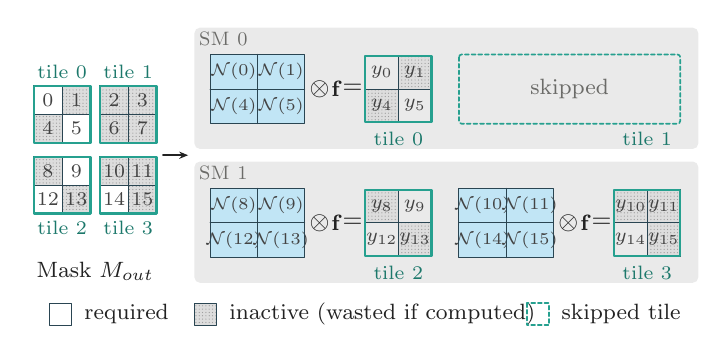
\begin{tikzpicture}[x=1mm, y=1mm]
  \def\isact#1{\pgfmathparse{or(or(or(or(#1==0,#1==5),#1==9),#1==12),#1==14)}}
  % \block{x}{y}{first index}{cell}{mode}: a 2x2 block of positions first, first+1, first+4, first+5;
  % mode 0 = mask (index), 1 = receptive fields N(p), 2 = issued outputs y_p; inactive positions dotted as in fig:masked-conv
  \newcommand{\block}[6]{% x, y, first index, cell width, cell height, mode
    \foreach \k/\o in {0/0, 1/1, 2/4, 3/5} {
      \pgfmathtruncatemacro\i{#3+\o}\pgfmathtruncatemacro\r{\k/2}\pgfmathtruncatemacro\q{mod(\k,2)}
      \ifnum#6=1 \fill[infill] (#1+\q*#4, #2-\r*#5) rectangle ++(#4, -#5);
        \node[idx, font=\fontsize{6.2}{6.4}\selectfont] at (#1+\q*#4+#4/2, #2-\r*#5-#5/2) {$\mathcal{N}(\i)$};
      \else \isact{\i}
        \ifnum\pgfmathresult=1 \actbox (#1+\q*#4, #2-\r*#5) rectangle ++(#4, -#5);
        \else \path[waste] (#1+\q*#4, #2-\r*#5) rectangle ++(#4, -#5); \fi
        \ifnum#6=2 \node[idx] at (#1+\q*#4+#4/2, #2-\r*#5-#5/2) {$y_{\i}$};
        \else \node[idx] at (#1+\q*#4+#4/2, #2-\r*#5-#5/2) {\i}; \fi
      \fi
    }
    \draw[rule, line width=0.35pt] (#1, #2) rectangle ++(2*#4, -2*#5) (#1+#4, #2) -- ++(0, -2*#5) (#1, #2-#5) -- ++(2*#4, 0);}
  \newcommand{\tframe}[3]{\draw[tileskip, line width=0.8pt] (#1, #2) rectangle ++(2*#3, -2*#3);}
  \newcommand{\tlabel}[3]{\node[idx, text=tileskip!75!black] at (#1, #2) {tile #3};}
  \def\aw{6.0}\def\ah{4.4}  % receptive-field cell
  \def\b{4.2}                % output cell
  % \issue{x}{y}{first index}{tile}: the tile's receptive fields (o) f = its outputs
  \newcommand{\issue}[4]{%
    \block{#1}{#2}{#3}{\aw}{\ah}{1}
    \node[op] at (#1+2*\aw+1.9, #2-\ah) {$\otimes$};
    \node at (#1+2*\aw+4.1, #2-\ah) {$\mathbf{f}$};
    \node[op] at (#1+2*\aw+6.1, #2-\ah) {$=$};
    \block{#1+2*\aw+7.7}{#2-\ah+\b}{#3}{\b}{\b}{2}\tframe{#1+2*\aw+7.7}{#2-\ah+\b}{\b}
    \tlabel{#1+2*\aw+7.7+\b}{#2-2*\ah-1.9}{#4}}
  % output mask in tiles
  \def\s{3.6}
  \def\my{-7.4}
  \block{0}{\my}{0}{\s}{\s}{0}\tframe{0}{\my}{\s}\tlabel{\s}{\my+1.8}{0}
  \block{8.4}{\my}{2}{\s}{\s}{0}\tframe{8.4}{\my}{\s}\tlabel{8.4+\s}{\my+1.8}{1}
  \block{0}{\my-9.0}{8}{\s}{\s}{0}\tframe{0}{\my-9.0}{\s}\tlabel{\s}{\my-9.0-2*\s-1.8}{2}
  \block{8.4}{\my-9.0}{10}{\s}{\s}{0}\tframe{8.4}{\my-9.0}{\s}\tlabel{8.4+\s}{\my-9.0-2*\s-1.8}{3}
  \node[title] at (7.8, -29.4) {Mask $M_{out}$};
  \draw[flow] (16.4, -16.2) -- (19.6, -16.2);
  % SMs (one per row), each issuing two tiles
  \def\sx{20.4}\def\sw{64.0}
  \fill[smfill, rounded corners=2pt] (\sx, 0) rectangle ++(\sw, -15.4);
  \fill[smfill, rounded corners=2pt] (\sx, -17.0) rectangle ++(\sw, -15.4);
  \node[smlabel] at (\sx, 0) {SM 0};
  \node[smlabel] at (\sx, -17.0) {SM 1};
  \issue{\sx+2.0}{-3.4}{0}{0}
  % tile 1: skipped (never issued)
  \draw[tileskip, line width=0.6pt, dash pattern=on 1.4pt off 1pt, rounded corners=1pt]
    (\sx+33.6, -3.4) rectangle ++(2*\aw+7.7+2*\b, -2*\ah);
  \node[text=muted] at (\sx+33.6+\aw+3.85+\b, -3.4-\ah) {skipped};
  \tlabel{\sx+33.6+2*\aw+7.7+\b}{-3.4-2*\ah-1.9}{1}
  \issue{\sx+2.0}{-20.4}{8}{2}
  \issue{\sx+33.6}{-20.4}{10}{3}
  % legend
  \begin{scope}[shift={(2.0, -35.0)}]
    \actbox (0, 0) rectangle ++(2.8, -2.8); \draw[rule, line width=0.35pt] (0, 0) rectangle ++(2.8, -2.8);
    \node[anchor=west] at (3.2, -1.4) {required};
    \path[waste] (18.4, 0) rectangle ++(2.8, -2.8); \draw[rule, line width=0.35pt] (18.4, 0) rectangle ++(2.8, -2.8);
    \node[anchor=west] at (21.6, -1.4) {inactive (wasted if computed)};
    \draw[tileskip, line width=0.6pt, dash pattern=on 1.4pt off 1pt] (60.6, 0) rectangle ++(2.8, -2.8);
    \node[anchor=west] at (63.8, -1.4) {skipped tile};
  \end{scope}
  \figframe{baseline}{Baseline: tile skipping}
\end{tikzpicture}
\end{document}
